\documentclass[letterpaper, 12pt]{article}
\usepackage[top=.5in,bottom=.5in,left=.75in,right=.75in,headheight=30pt, % as per the warning by fancyhdr
includehead,includefoot,
heightrounded, % to avoid spurious underfull messages
]{geometry}
\addtolength{\topmargin}{-.25in}
\usepackage{fancyhdr}
\pagestyle{fancy}
\usepackage{graphicx}
\usepackage{lastpage}
\usepackage{multicol}
\usepackage{qrcode}
\usepackage{gensymb}
\usepackage{pgfplots}

\begin{document}
\fancyhead[l]{	
\includegraphics[height=0.5in]{../Logo/sp.png} Name:}
\fancyhead[r]{Due Date: \hspace{ 1in}}
\fancyfoot[c]{\thepage\ of \pageref{LastPage}}
\fancyfoot[r]{Assignment 3.01}	


\begin{center} Assignment 3.01: Position vs Time Graphs

\vspace{0.1in}
	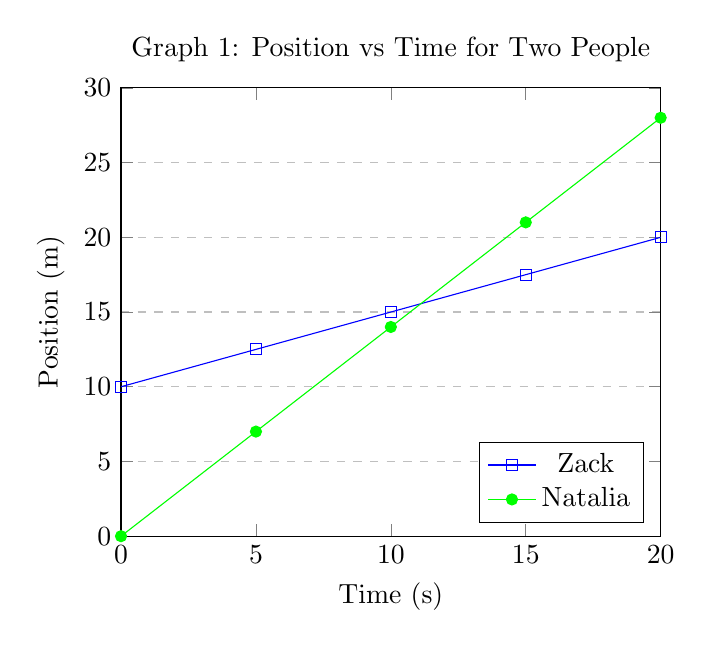
\begin{tikzpicture}
\begin{axis}[
title={Graph 1: Position vs Time for Two People},
xlabel={Time (s)},
ylabel={Position (m)},
xmin=0, xmax=20,
ymin=0, ymax=30,
xtick={0,5,10,15,20},
ytick={0,5,10,15,20,25,30},
ymajorgrids=true,
grid style=dashed,
legend pos=south east,
]

\addplot[
color=blue,
mark=square,
]
coordinates {
	(0,10)(5,12.5)(10,15)(15,17.5)(20,20)};
\addlegendentry{Zack}

\addplot[
color=green,
mark=*,
]
coordinates {
	(0,0)(5,7)(10,14)(15,21)(20,28)};
\addlegendentry{Natalia}



\end{axis}
\end{tikzpicture}
\end{center}


\begin{enumerate}
 \item  \vspace{-.2in} Use Graph 1 to determine the following: \vspace{-.1in}
\begin{enumerate}
	\item Where is Zack located at t=5 seconds? \vspace{.25in}
	\item Without calculating speeds, who is moving faster, Zack or Natalia?  Explain your \\ reasoning.\vspace{.25in}
	\item What is Zack's Speed?\vspace{.25in}
	\item What is Natalia's Speed?\vspace{.25in}
	\item What is Zack's Acceleration?\vspace{.25in}
	\item Who starts ahead, Zack or Natalia?  Explain your reasoning.\vspace{.25in}
	\item Who ends ahead, Zack or Natalia?  Explain your reasoning.\vspace{.25in}
	\item Who has the greater acceleration, Zack or Natalia?  Explain your reasoning. \vspace{.25in}
	\item Graph 1 describes a race between Zack and Natalia.  In at least 4 complete sentences, describe what happened during this race. \vspace{1in}
\end{enumerate}

\begin{center}
	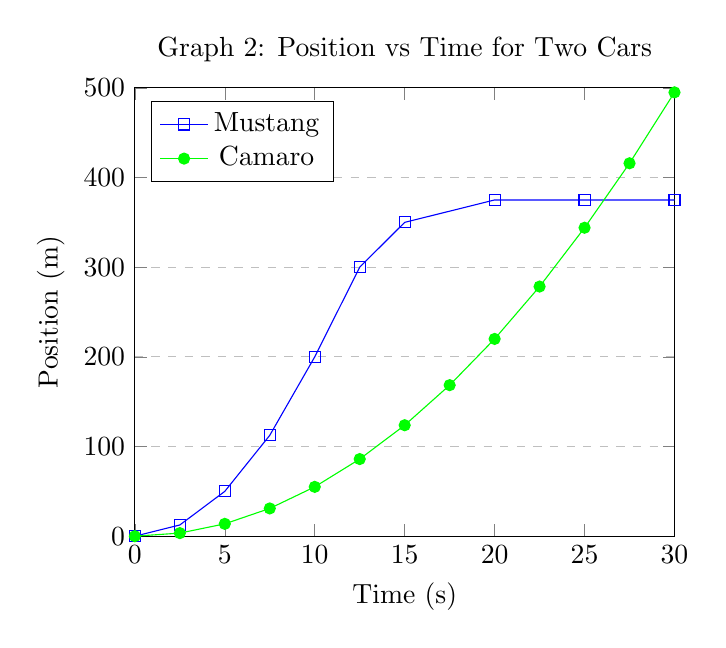
\begin{tikzpicture}
\begin{axis}[
title={Graph 2: Position vs Time for Two Cars},
xlabel={Time (s)},
ylabel={Position (m)},
xmin=0, xmax=30,
ymin=0, ymax=500,
xtick={0,5,10,15,20,25,30},
ytick={0,100,200,300,400,500},
ymajorgrids=true,
grid style=dashed,
legend pos=north west,
]

\addplot[
color=blue,
mark=square,
]
coordinates {
	(0,0)(2.5,12.5)(5,50)(7.5,112.5)(10,200)(12.5,300)(15,350)(20,375)(25,375)(30,375)}; 
\addlegendentry{Mustang}

\addplot[
color=green,
mark=*,
]
coordinates {
	(0,0)(2.5,3.43)(5,13.75)(7.5,30.94)(10,55)(12.5,86)(15,123.75)(17.5,168.4375)(20,220)(22.5,278.4)(25,344)(27.5,415.9)(30,495)};
\addlegendentry{Camaro}



\end{axis}
\end{tikzpicture}
\end{center}
\item Use the Graph 2 to answer the following questions:
\begin{enumerate}
	\item Which car has the greater acceleration during the first 10 seconds?\vspace{.25in}
	\item Which car slows down and stops?\vspace{.25in}
	\item Which car is traveling faster at t=10 seconds?\vspace{.25in}
	\item Which car is traveleing faster at t=20 seconds?\vspace{.25in}
	\item This graph describes a race between two cars that are racing 400 meters (approximately $\frac{1}{4}$ of a mile).  In a paragraph of at least 5 sentences, explain what happens during the race.

\end{enumerate}	

\pagebreak

	\item Describe the motion that would result in the following graphs:
	
	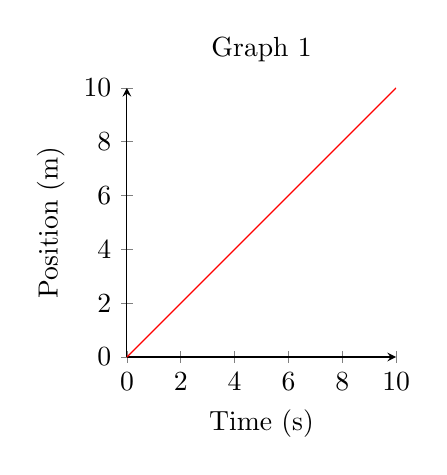
\begin{tikzpicture}
	\begin{axis}[title=Graph 1, xlabel=Time (s), ylabel=Position (m), axis lines = left, width=5cm,height=5cm]
	% density of Normal distribution:
	\addplot
	[
	red,
	domain
	=0:10,
	samples
	=201,
	]
	{x};
	\end{axis}
	\end{tikzpicture}%
	%
	%
	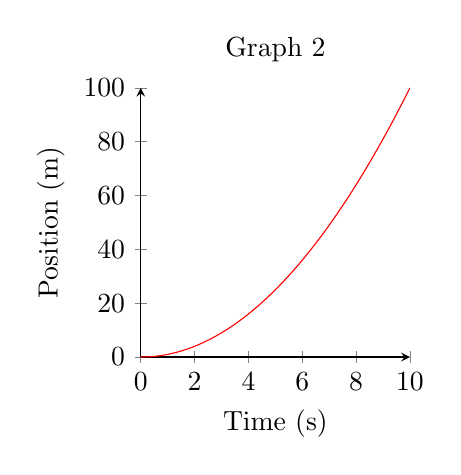
\begin{tikzpicture}
	\begin{axis}[title=Graph 2, xlabel=Time (s), ylabel=Position (m), axis lines = left, width=5cm,height=5cm]
	% density of Normal distribution:
	\addplot
	[
	red,
	domain
	=0:10,
	samples
	=201,
	]
	{x^2};
	\end{axis}
	\end{tikzpicture}%	
	%
	%
	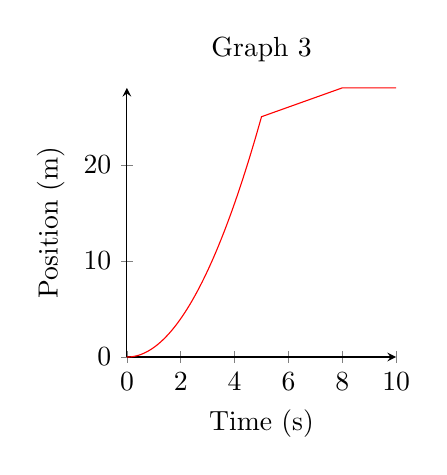
\begin{tikzpicture}[declare function={
		func(\x)= (\x<=5) * (\x^2)   +
		and(\x>5,  \x<=8) * (\x+20) +
		(\x>8) * (28);
	}]
	\begin{axis}[title=Graph 3, xlabel=Time (s), ylabel=Position (m), axis lines = left, width=5cm,height=5cm]
	% density of Normal distribution:
	\addplot
	[
	red,
	domain
	=0:10,
	samples
	=201,
	]
	{func(x)};
	\end{axis}
	\end{tikzpicture}%


\begin{enumerate}
	\item Graph 1: \vspace{0.3in}
	\item Graph 2:\vspace{0.3in}
	\item Graph 3:\vspace{0.3in}
	
	\end{enumerate}

\item Sketch a graph that corresponds to each situation below:
\begin{enumerate}
	\item A car is parked.
	\item A truck drives forward 10 meters at a constant speed, then stops.
	\item A lion runs forward, then stops, then walks back to where it started.
\end{enumerate}

	\begin{tikzpicture}
\begin{axis}[title=(a), xlabel=Time (s), ylabel=Position (m), axis lines = left, width=5cm,height=5cm,  ymin=0, ymax=10]
% density of Normal distribution:
\addplot
[
red,
domain
=0:10,
samples
=201,
]
{0};
\end{axis}
\end{tikzpicture}%
%
%
\begin{tikzpicture}
\begin{axis}[title=(b), xlabel=Time (s), ylabel=Position (m), axis lines = left, width=5cm,height=5cm, ymin=0, ymax=10]
% density of Normal distribution:
\addplot
[
red,
domain
=0:10,
range=0:10,
samples
=201,
]
{0};
\end{axis}
\end{tikzpicture}%	
%
%
\begin{tikzpicture}[]
\begin{axis}[title=(c), xlabel=Time (s), ylabel=Position (m), axis lines = left, width=5cm,height=5cm, ymin=0, ymax=10]
% density of Normal distribution:
\addplot
[
red,
domain
=0:10,
samples
=201,
]
{0};
\end{axis}
\end{tikzpicture}%


\end{enumerate}
\end{document}
